\let\negmedspace\undefined
\let\negthickspace\undefined
\documentclass[journal,12pt,onecolumn]{IEEEtran}
\usepackage{cite}
\usepackage{amsmath,amssymb,amsfonts,amsthm}
\usepackage{algorithmic}
\usepackage{graphicx}
\graphicspath{{Figs/}}
\usepackage{textcomp}
\usepackage{xcolor}
\usepackage{txfonts}
\usepackage{listings}
\usepackage{enumitem}
\usepackage{mathtools}
\usepackage{gensymb}
\usepackage{comment}
\usepackage{caption}
\usepackage[breaklinks=true]{hyperref}
\usepackage{tkz-euclide} 
\usepackage{listings}
\usepackage{gvv}                                        
%\def\inputGnumericTable{}                                 
\usepackage[latin1]{inputenc}     
\usepackage{xparse}
\usepackage{color}                                            
\usepackage{array}                                            
\usepackage{longtable}                                       
\usepackage{calc}                                             
\usepackage{multirow}
\usepackage{multicol}
\usepackage{hhline}                                           
\usepackage{ifthen}                                           
\usepackage{lscape}
\usepackage{tabularx}
\usepackage{array}
\usepackage{float}
%\newtheorem{theorem}{Theorem}[section]
%\newtheorem{theorem}{Theorem}[section]
%\newtheorem{problem}{Problem}
%\newtheorem{proposition}{Proposition}[section]
%\newtheorem{lemma}{Lemma}[section]
%\newtheorem{corollary}[theorem]{Corollary}
%\newtheorem{example}{Example}[section]
%\newtheorem{definition}[problem]{Definition}

\begin{document}

\title{Signed Distances}
\author{AI25BTECH11002 - Ayush Sunil Labhade}
{\let\newpage\relax\maketitle}
%\renewcommand{\thefigure}{\theenumi}
%\renewcommand{\thetable}{\theenumi}
A line is represented by the equation $\vec{n}^T\vec{x}=c$ where n is the normal vector, x is a point on the line and c is an arbitrary constant. 
The normal vector is perpendicular to the line and for more intuitive understanding it can be represented as:
\begin{figure}[H]
	\centering
	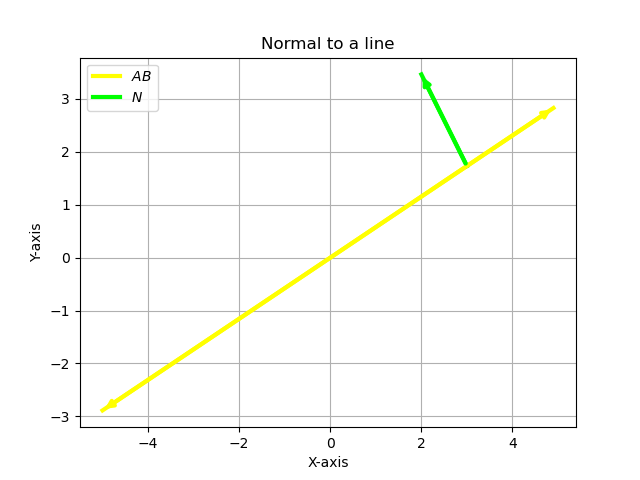
\includegraphics[scale=0.5]{norm}
	\caption{}
	\label{fig1}
\end{figure}
The direction of the normal has only two possiblities as shown:
\begin{figure}[H]
	\centering
	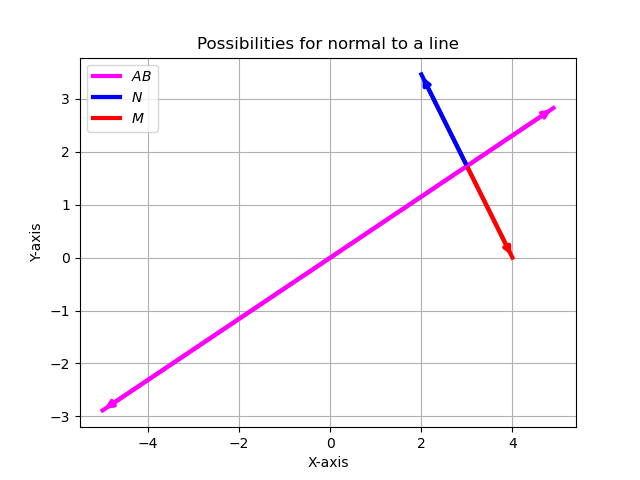
\includegraphics[scale=0.5]{binorm}
	\caption{}
	\label{fig2}
\end{figure}
The exact direction of the normal can be determined by the equation of line and substituting a known point $\brak{usually \ \vec{x}=\myvec{0 \\ 0}}$ and using the concept of signed distance which is discussed further.
\begin{align}
\vec{n}^T\vec{x}-c=0
\end{align}
\begin{align}
 \brak{\vec{n}^T\vec{0}-c}>0 \ or \ \brak{\vec{n}^T\vec{0}-c}<0 
\end{align}
Respective normals in both the cases:
\begin{figure}[H]
	\centering
	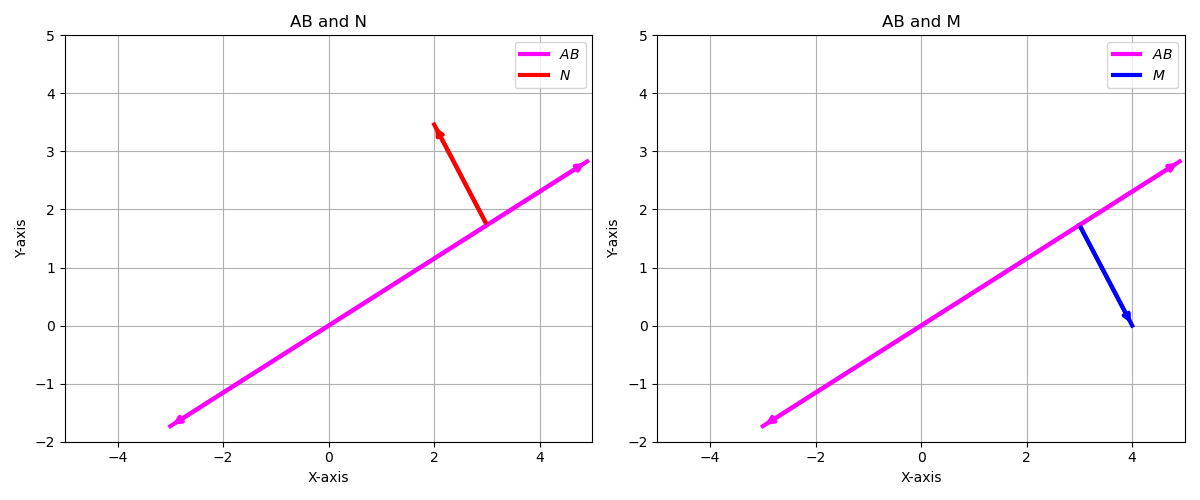
\includegraphics[scale=0.5]{normal}
	\caption{}
	\label{fig3}
\end{figure}
Suppose one of the cases, the direction of normal would be fixed. Here the term $\vec{n}^Tx-c$ is basically the dot product of any arbitrary $\vec{x}$ with the normal vector.(c is just a constant representing shifting) 
Here two cases arise:
\begin{enumerate}
\item When the point x is on the same side as normal, the dot product is positive, and hence the term $$\brak{\vec{n}^T\vec{x}-c}>0$$ 
\item When the point x is on the opposite side of normal, the dot product is negative, and hence the term $$\brak{\vec{n}^T\vec{x}-c}<0$$
\end{enumerate}
Hence when two vectors $\vec{A} \ and \ \vec{B}$ are on opposite side, the condition $$\brak{\vec{n}^T\vec{A}-c}\brak{\vec{n}^T\vec{B}-c}<0 $$ is sufficient and necessary.
\end{document}
